\chapter{Analisi del problema}

\epigraph{"There were 5 exabytes of information created between the dawn of civilization through 2003, but that much information is now created every 2 days."}{\textit{Eric Schmidt (Google), 2010}}

%delete justify
\begin{flushleft}
\end{flushleft}
Un problema particolarmente noto e più che mai attuale riguarda i dati. La mole di dati che è collezionata quotidianamente nel mondo è inverosimile. Come ogni applicazione, servizio o sistema, anche SeismoCloud è sommersa costantemente da essi. La quantità ricevuta, come si denoterà di seguito, necessita di una riorganizzazione nel modo in cui essi sono collezionati, di come sono fruiti e dell'utilità che essi possono fornire in ambito interno ed esterno.

\section{Una nuova architettura per la collezione dei dati} \label{previousarch}

Uno dei flussi più imponente di dati riguarda le informazioni inviate periodicamente dai sensori: essendo essi gli strumenti di rilevazione di terremoti, elementi quindi imprescindibili per il corretto funzionamento interno del sistema nella sua totalità, è sempre importante monitorare ed acquisire sia gli aspetti più immediati dal punto di vista logico (quindi eventi sismici rilevati, posizione geografica per attribuire a questi ultimi un luogo), sia aspetti di apparente importanza superficiale, che di superficiale, in una prospettiva temporale ampia, hanno poco. Alcuni esempi sono la temperatura del sismometro, il suo indirizzo IP e l'alimentazione.

\paragraph{La quantità di dati}
L'aspetto cruciale che permette di quantificare come imponente la quantità di dati registrata dai sensori è il periodo di trasmissione: ogni dato viene difatti spedito ogni 5 minuti. Considerando un time frame giornaliero di 24 ore, si ha che il numero di trasmissioni per sensore è pari a:
\begin{equation} \label{eq:dailytrans}
transmissions = \frac{timeFrame}{sendingInterval} 
= \frac{24 * 60\ minutes}{5\ minutes} 
= 288\ transmissions
\end{equation}
Si consideri, inoltre, che i dati inviati per trasmissione sono i seguenti:\\
temperature, rssi, publicip, localip, threshold, bssid, essid.
Si immagini dunque come ogni giorno ciascun sensore produca 288 valori di ognuno degli elementi di cui sopra, non considerando i segnali di liveness che essi inviano ogni di 14 minuti (dato che, nel calcolo precedente, è stato trascurato). Ad essi si aggiungano un timestamp, per tenere traccia del momento dell'invio dei dati, e l'ID dei Sismometri, e si giunge ad un numero di dati inviato quotidianamente pari a:
\begin{equation} \label{eq:dailyoneseismo}
\begin{split}
dataSent = transmissions * len(elements) = \\
= 288\ transmissions * 9\ elements = 2592\ single\ elements\ sent
\end{split}
\end{equation}
dove, per \textit{len(elements)}, si intende il numero di elementi inviati dai sensori, quindi sommando singolarmente i dati quali temperature, rssi, ecc.\\
Come ultimo calcolo dimostrativo, si prenda come ipotesi che il numero di device attivi siano 100 (dato che rispecchia il numero attualmente attivo di device). Con una semplicissima moltiplicazione, si ottiene che il numero di dati ricevuti \textbf{ogni giorno} da SeismoCloud sono pari a:
\begin{equation} \label{eq:overalldailytrans}
dailyData = singleSeismoData * activeSeismos = 2592 * 100 = 259.200\ elems
\end{equation}
Appare quindi chiara la necessità di inserire i dati ricevuti in un nuovo sistema a sé stante, \textit{scalabile} e \textit{data-oriented}.

\paragraph{Il sistema attuale}
L'architettura del sistema, in una versione ad alto livello è rappresentata nella Figura \ref{fig:datainsertionmaria}.
Il collezionamento dei dati si articola nei seguenti passi:
\begin{itemize}
    \item I sensori inviano dati tramite il protocollo MQTT (Message Queue Telemetry Transport) \cite{mqtt} al Broker MQTT.
    \item Il Broker comunica con un controller.
    \item Il controller inserisce i dati nel database MariaDB. 
    \item I dati sono salvati nel database.
\end{itemize}
Il problema principale individuato è il salvataggio dei dati:\\
in primo luogo, il controller comunica direttamente con il database, inserendo in modo sincrono i dati. Un cambiamento di database comporterebbe una modifica nel controller;
in secondo luogo, i dati sono inseriti in un database che non ha una particolare predisposizione ai dati che rappresentano serie temporali di elementi, come quelli in esame. 
\begin{figure}[h]
    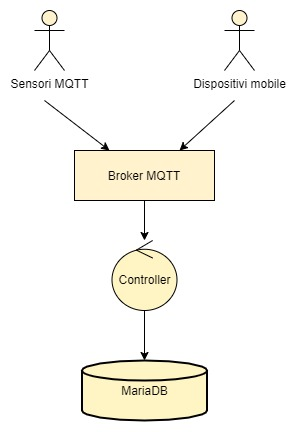
\includegraphics[scale=0.67, center]{images/insertdatamaria.jpg}   
    \caption{Architettura attuale per la gestione dei dati dei sensori.}
    \label{fig:datainsertionmaria}
\end{figure} 

\section{API per i dati storici} \label{apidatistorici}

\paragraph{Fornire dati agli utenti}
Le informazioni collezionate dai sensori sono disponibili solo internamente al sistema, o, eventualmente, su richiesta. Si vuole permettere ad utenti esperti di usufruirne per effettuare statistiche su di essi, indirizzarli al training di algoritmi di ML, o altre utilità che possano trovare.\\
Un accesso libero, tuttavia, non è assolutamente una soluzione ammissibile: permettere ad un utente (senza alcuna autenticazione) di richiedere \textbf{potenzialmente} ogni dato relativo ai sensori contenuto all'interno del database non solo gli permetterebbe di clonarli, manipolarli e distribuirli a suo piacimento, ma, come caso limite, porterebbe ad un possibile denial of service, in quanto impegnerebbe il server con una query con un risultato di dimensione notevole.\\
Un altro approccio considerato prevede la creazione di un set di API per soddisfare le richieste in modo controllato, ben delimitato nello span delle richieste possibili.
Quest'ultimo approccio è stato prediletto per l'esternazione dei dati.

\paragraph{Quali dati fornire ed entro quali limiti} 
Sulla base di quanto osservato in \ref{previousarch}, considerando inoltre il target principale delle API, si è scelto di fornire agli end user un subset delle informazioni inviate dai sensori, classificabili nelle due seguenti categorie:
\begin{itemize}
    \item Informazioni sullo status di alcune funzioni vitali del sensore
    \item Informazioni sulle scosse rilevate
\end{itemize}
In particolare, sul primo elemento si è stabilito di rendere disponibili dati quali la \textbf{Temperatura} del sismometro, il \textbf{RSSI} (Received Signal Strength Indication) ed il parametro di \textbf{Threshold}. \\
Per la maggior parte dei parametri l'importanza non risiede nel singolo valore degli stessi in un determinato istante di tempo, ma risultano estremamente più utili se analizzati in un periodo esteso. Un esempio lampante è l'analisi dei valori della temperatura del sensore in un periodo pari all'ultimo mese o anno, dati che potrebbero aiutare a prevenire un eventuale surriscaldamento prolungato (e conseguente rottura) di un dispositivo, permettendo al proprietario di installare un dispositivo di raffreddamento più adeguato o di programmarne lo spegnimento in determinate occasioni. Un discorso del tutto analogo può essere fatto per l'utilità degli altri dati.\\
Deve essere quindi possibile richiedere i dati specificando un range temporale.\\
In ultimo luogo, un criterio determinante per la selezione dei dati è per quali sensori effettuare la richiesta: ogni utente possiede l'identificativo dei propri sensori, per cui la richiesta dei relativi dati appare naturale.
Potrebbe essere però interessante (oltre che importante) richiedere i dati relativi ad una certa posizione geografica, estesa entro un certo raggio. Questa opzione, quindi, deve essere inclusa nella fase successiva di design.

\paragraph{Come fornire i dati}
Vista l'utilità che i dati dei Sismometri rappresentano, sarebbe piuttosto scomodo lato utente ricevere una risposta HTTP contenente tutti i risultati in formato \textbf{JSON} (JavaScript Object Notation) \cite{json}, come usualmente è effettuato in SeismoCloud per altri tipi di richieste: sarebbe invece più utile avere a disposizione i risultati all'interno di un file. Il formato del file in questione deve essere scelto in accordo con il suo possibile impiego: il formato \textbf{CSV} può essere particolarmente utile per consentire agli utenti di trasferire i dati ottenuti direttamente su fogli di calcolo, come \textbf{Excel} \cite{excel}, o per essere usati con librerie come \textbf{Pandas} \cite{pandas} per l'analisi dei dati. Un altro formato da rendere disponibile è il \textbf{GeoJSON} \cite{geojson}, formato di rappresentazione di oggetti geospaziali, con le loro proprietà e caratteristiche, basato su JSON. Ancora, un formato che potrebbe espandere l'utilizzo che si ha di questi dati è il \textbf{HDF5} \cite{hdf5}, usato, tra le altre cose, nel campo del Machine Learning (un esempio è la richiesta di utilizzare questo formato per il salvataggio di modelli \cite{tensorflow}). Infine, una ultima scelta da parte dell'utente può essere \textbf{MiniSeed} \cite{miniseed}, il cui acronimo sta per "mini Standard for the Exchange of Earthquake Data", per cui, per i dati relativi soprattutto alle scosse sismiche, sembra più che adatto. 

\section{Il tempo di una richiesta} \label{moledati}
Nella sezione \ref{apidatistorici} si è discusso circa i dati che il sistema dovrà fornire e le motivazioni principali legate all'utilizzo delle API. \\
Facendo riferimento ad un possibile Use Case di analisi statistica dei dati su un intervallo di anche solo un mese per un certo numero di Sismometri, è facile notare (facendo anche riferimento ai calcoli mostrati nell'equazione \ref{eq:dailyoneseismo} per un solo Sismometro) come la mole di informazioni da trasferire sia non indifferente.
Di fronte a queste cifre, ci si attende che il sistema non riesca ad elaborare ogni richiesta in maniera immediata, fornendo all'utente in modo sincrono tutti i dati richiesti. Una soluzione potrebbe essere ignorare la problematica e supporre che l'utente sia disposto ad attendere che la richiesta sia completata, ma ciò appare un modo di aggirare il problema piuttosto che risolverlo. Una soluzione più accurata prevede che la richiesta sia soddisfatta in modo \textbf{asincrono}, facendo in modo che l'utente possa effettuare una richiesta e poi essere libero di non attendere una risposta, mentre il sistema, internamente, la elabora. Le API devono essere quindi progettate per essere \textit{asincrone}: l'utente deve poter effettuare una richiesta ed essere in grado, una volta pronti i file, di ottenere i risultati. Deve quindi essere pensato sia un meccanismo di notifiche che notifichi l'utente nel momento in cui i risultati sono disponibili, sia un modo di accedere ai risultati stessi.

\paragraph{Back End ottimizzato}
Il fatto che si sia stabilito che le API siano asincrone non deve tuttavia rilassare i vincoli sul tempo di esecuzione di ogni richiesta: non ottimizzare il codice che verrà utilizzato per il Back End del sistema significa aumentare il tempo di risposta per un utente; inoltre, con poche accortezze, si rischia di sovraccaricare il server su cui il codice verrà installato con del lavoro inutile, portando a possibili failure dello stesso in caso di richieste a carico elevato o in caso di risorse non chiuse correttamente. Deve altresì essere possibile stabilire un tetto massimo di esecuzione, a livello temporale, per evitare di ricadere in richieste sottilmente volte all'estrazione di una quantità di dati spropositata, modellando in modo subdolo i parametri già discussi in \ref{apidatistorici}. 